\documentclass[titlepage, 11pt]{article}
%\usepackage{showframe}
\usepackage[a4paper, nomarginpar, total={170mm,257mm, left=25mm, right=15mm, top=20mm,bottom=20mm}]{geometry}

\title{Lyčių nelygybė visuomenėje: kaip tai pasireiškia šeimoje?}
\author{Angelina Beliajeva}



\usepackage[utf8]{inputenc}
\usepackage[L7x]{fontenc}
\usepackage[lithuanian]{babel}
\usepackage{textcomp}

\usepackage{tgtermes}
\usepackage{indentfirst}

\usepackage{graphicx}
\usepackage{float}
\usepackage{caption}


\usepackage{hyperref}
\hypersetup{
colorlinks=true,
linkcolor=black,
filecolor=black,
urlcolor=blue,
citecolor=black
}

\usepackage{setspace}
\onehalfspacing
\usepackage[
backend=biber,
style=apa,
url=false,
sorting=nyt,
]{biblatex}

\addbibresource{literatura.bib}

\begin{document}
\maketitle
\tableofcontents
\newpage
\section{Įvadas}

Žmonijos susiskaidymas į dvi puses tapo daugelių ilgai besitęsiančių ginčų pradžia. Vienas iš jų yra susijęs su lyčių nelygybe ir klausimu, ar vyrai ir moterys iš esmės yra vienodi, ar iš esmės yra skirtingi. Iki šiol visuomenėje vyrauja dar senais laikais nusistovėję stereotipai, kad moteris turi būti nukreipiama į šeimą, vaikų auklėjimą ir auginimą, o vyras - į fizinį aktyvumą, vadovavimą ir intelektualinį darbą. Galimybes gyvuoti visuomenėje šiems stereotipams suteikia kultūra, pasitelkdama įvairias visuomenines sferas: meną, religiją, politiką, ekonomiką. Kadangi stereotipai, kurie moko mus būti vyrais ir moterimis, yra perduodami iš kartos į kartą, lyčių nelygybę sustabdyti yra sunku. Tai lemia vyrų dominavimą, tačiau moterų nuvertinimą tiek visuomeniniame, tiek asmeniniame gyvenimuose.

\section{Kas yra lyčių nelygybė?}

Lyčių nelygybė gali būti paaiškinama kaip nevienodas požiūris į asmenį, jo gebėjimus, veiksmus, suvokimą pagal lytį. Lyčių nelygybė dar yra vadinama seksizmu – „žmonių diskriminacija ir neapykanta dėl jų lyties, ignoruojant kitas asmens savybes. Paprastai siejama su bet kokiu asmens išskyrimu ar vertinimu, remiantis vien jo lytimi.“ Šioje sąvokoje slypi gyli mintis, kad vienos arba kitos lyties atstovas yra kuo nors geresnis, svarbesnis arba vertingesnis.

\section{Kokios yra lyčių lygybės kliūtys?}

Egzistuoja daugybė veiksnių, trukdančių sustabdyti lyčių nelygybės problemą visuomenėje. Vienas tokių – sunkiai besikeičiantis, nusistovėjęs žmonių mentalitetas. Tokiu būdu „Tradiciniais lyčių vaidmenimis paremta ideologija susieja moterį su privačiąja sfera, jai užkraunama atsakomybė ir pareigos dirbti nemokamą globos darbą, ji priklausoma darbo rinkos ir viešosios sferos atžvilgiu, tampa priklausoma nuo pajamas gaunančio vyro bei taip apribojamos jos galimybės realizuoti savo socialines teises“ \cite{maslauskiene2004globa}. Trumpai tariant, moteris nukreipiama į ramią vidinę aplinką, t.y., šeimą, vaikų auklėjimą, globą. Priešingai, vyras dažniausiai yra vaizduojamas kaip pagrindinė figūra pasaulyje. Dauguma teigia, kad būtent vyrai visais laikais buvo žymūs, sėkmingi tyrinėtojai, architektai, statytojai, verslininkai, politikai, taip smarkiai pakeitę pasaulį, kad kartais atrodo, jog moterų nuopelnai, išgyvenami sunkumai, pavyzdžiui, darbščiai bei sunkiai siekiant gerų rezultatų karjeroje, apskritai atrodo nesvarbūs. Būtent vyrus tradiciškai aprašo kaip „sėkmingai lipančius karjeros laiptais ir išlaikančius šeimą“ \cite{maslauskiene2004globa}. Tokiu būdu ir iki šių dienų vyrauja nuomonė, kad pirmaujančias pozicijas darbe, šeimoje ir apskritai visuomenėje užima vyrai, o moterys – pavaldžias. Kitas veiksnys, griaunantis lyčių nelygybės panaikinimo procesą, yra lyčių stereotipai. Skiriami du stereotipų tipai: aprašomieji ir nurodantieji.
\begin{enumerate}

\item  („Aprašomieji stereotipai – tai skirtingų lyčių atstovams priskiriamos tipiškai skirtingos ir priešingos savybės“ \cite{Reinikovaite1998zmogus} ). Teigiama, kad vyriškumo savybės tai – aktyvumas, jėga, išvystytas loginis mąstymas, dominavimas, kontrolė. Dažniausiai iš vyrų tikimasi sėkmės viešojoje aplinkoje. Štai moterims, manoma, kad būdinga būti pasyvioms, neveiklioms, pažeidžiamoms, silpnoms ir atliekančioms „dekoracijų“ funkciją. Paprastai,  jeigu moteris dirba viešojoje sferoje, tai numanoma, kad ji dirba tradicinį „moterišką“ darbą, pavyzdžiui, mokytojos, sekretorės arba auklėtojos. 
\item („Nurodantieji stereotipai – nusakantys, kaip privalo elgtis vienos ar kitos lyties atstovai“ \cite{Reinikovaite1998zmogus}). Todėl yra atskiriamas tinkamas elgesys vyrams ir moterims. Pavyzdžiui, daugumos pažįstama situacija, kad mergaites tėvai auklėja ir prižiūri griežčiau nei berniukus, aiškindami, kaip elgtis pridera, o kaip ne. Kitaip tariant, nuo pat vaikystės žmonėms yra skiriami tam tikri vaidmenys. Tai yra susiję su rožine bei žydra spalva, dovanojamomis lėlėmis bei žaisliniais automobiliais ir kitais mergaitėms ir berniukams skirtais daiktais.
\end{enumerate}
Taigi, anksčiau paminėti aspektai nesąmoningai ugdo žmoguje tam tikras taisykles – moterys nuo pat vaikystės kreipiamos į ramų, pasyvų elgesį bei vidinę sferą, o vyrai į išorinę, daug aktyvesnę. Tokiu būdu ir pamažu gimsta faktoriai, trukdantys įgyvendinti lyčių lygybės egzistavimą visoje visuomenėje.

\section{Kaip visuomenėje suprantama tradicinės šeimos sąvoka ir kaip ji pakito šiuolaikiniame pasaulyje?}

Šeima – vieną svarbiausių daugumos žmonių vertybių. Todėl šeimos sąvoka ir jos supratimas yra labai svarbūs visai visuomenei. Paprastai, šeima yra vaizduojama kaip dviejų susituokusių žmonių, turinčių vaikų, pastovų darbą, bendrą buitį, aplinka. Ne paslaptis, kad šeimoje išskiriamas vienas svarbiausias, už viską atsakingas asmuo – dažniausiai tai – vyras. Jis yra įstatymo, pareigos įsikūnijimas, turintis teisę spręsti, bausti, atleisti, įsakyti. Visai kitokia yra moterų padėtis šeimoje. Analizuojant tradiciškos šeimos sąvoką pastebima, kad labiausiai vertinama moteris (šeimoje) yra kantri, prisitaikanti prie bet kurios situacijos bei savarankiškai nepriimanti sprendimų. Trumpai tariant, moterys yra laikomos namų šeimininkėmis, o vyrai – šeimos „vadovais“.\newline
Toks vyrų ir moterų savybių paskirstymas, deja, sukuria pamatą įsivyrauti lyčių nelygybei ir šeimyniniame gyvenime. Vyrų išaukštinimas šeimoje dažniausiai, patiems vyrams nesuvokiant, priverčia juos piktnaudžiauti savo padėtimi ir nuvertinti moteris. \newline
Tiesa, šiuolaikinėje visuomenėje pamažu yra naudojamos naujos, lyčių lygybe gristos, šeimos sąvokos: „simetrinis šeimos modelis“ arba „dviejų karjerų“ šeima. Šių reikšmių pagrindinė mintis yra ta, kad abiem iš tėvų pridera vienodai dirbti ir rūpintis vaikais bei šeimos buitimi. Esant tokiems šeimos modeliams atsiranda lyčių papildomumas – „vyriškas ir moteriškas lygiavertis bendradarbiavimas“ – kurio siekti pridera kiekvienai šeimai. Galima teigti, kad gyventi pagal paminėtus šiuolaikiškus šeimos modelius yra vienas iš būdų panaikinti lyčių nelygybę, kadangi kiekvienas iš sutuoktinių turėtų panašesnes/vienodas pareigas, kurios suteiktų galimybę abiem žmonėms žvelgti į vienas kitą su tam tikra pagarba.

\section{Kaip lyčių nelygybė pasireiškia šeimyniniame gyvenime?}

Nepaisant anksčiau paminėtų aspektų, lemiančių lyčių nelygybės situaciją šeimoje, egzistuoja dar trys, ne mažesnio dėmesio verti, faktoriai, susiję su analizuojama problema, t.y., vyrų ir moterų darbo užmokesčio skirtumai, užimamos pareigos darbe ( darbo pobūdis ) ir moterų išgyvenama dilema siekiant skirti vienodai laiko tiek vaikų auginimui, tiek karjerai.

\begin{enumerate}
\item Ne paslaptis, kad vienas aršiausių ginčų tarp moterų ir vyrų kyla dėl darbo užmokesčio skirtumo. Remiantis EUROSTAT duomenimis, skirtumas tarp moterų ir vyrų atlyginimo pradėjo didėti nuo 2011 m. ir iki šiol nemažėja. Teigiama, kad viena iš priežasčių, dėl kurios moterys gauna mažiau pajamų – gaunamos apmokamos atostogos vaikų priežiūrai bei įmonių teikiamos kitos socialinės paramos. Todėl „tokia darbuotoja dažnokai yra nepatraukli verslui, rinkai ir darbdaviui“ \cite{Reinikovaite1998zmogus}, nes reikalingos papildomos išlaidos. ( Tokiu būdu, kol vyrai kyla karjeros laiptais, pretenduoja gauti didesnį atlyginimą, moterys įgyja didžiulę spragą darbo sferoje ir po to sunkiai grįžta į senąsias vėžes. ) Taip pat, būtina paminėti, kad vyrų ir moterų atlyginimo skirtumai yra glaudžiai susiję su rinkos segregacija tarp vyrų ir moterų – profesijų paskirstymas tarp vyrų ir moterų. Ši situacija yra sutinkama visuomenėje dėl žmonėse glūdinčių senais laikais atsiradusių stereotipų apie moterų ir vyrų profesijas. Ne retai yra girdima, kad moterys dirba „menkesnės vertės darbą“ - slaugos, rūpybos, valymo, mokymo ir kt. – „žinoma, už juos mokama mažiau“. Tokiu būdu, galima teigti, kad dėl asmeniniams gyvenimui tiekiamų paslaugų bei įsišaknijusių lyčių stereotipų, yra nepakankamai vertinamas moterų potencialas bei darbo galimybės, o tai lemia vyrų ir moterų atlyginimų skirtumo didėjimą.

Pavaizduotas grafikas parodo bendrą vaizdą apie lyčių nelygybę darbo užmokesčio srityje.

\begin{figure}[H]
\captionsetup{justification=centering}
\center
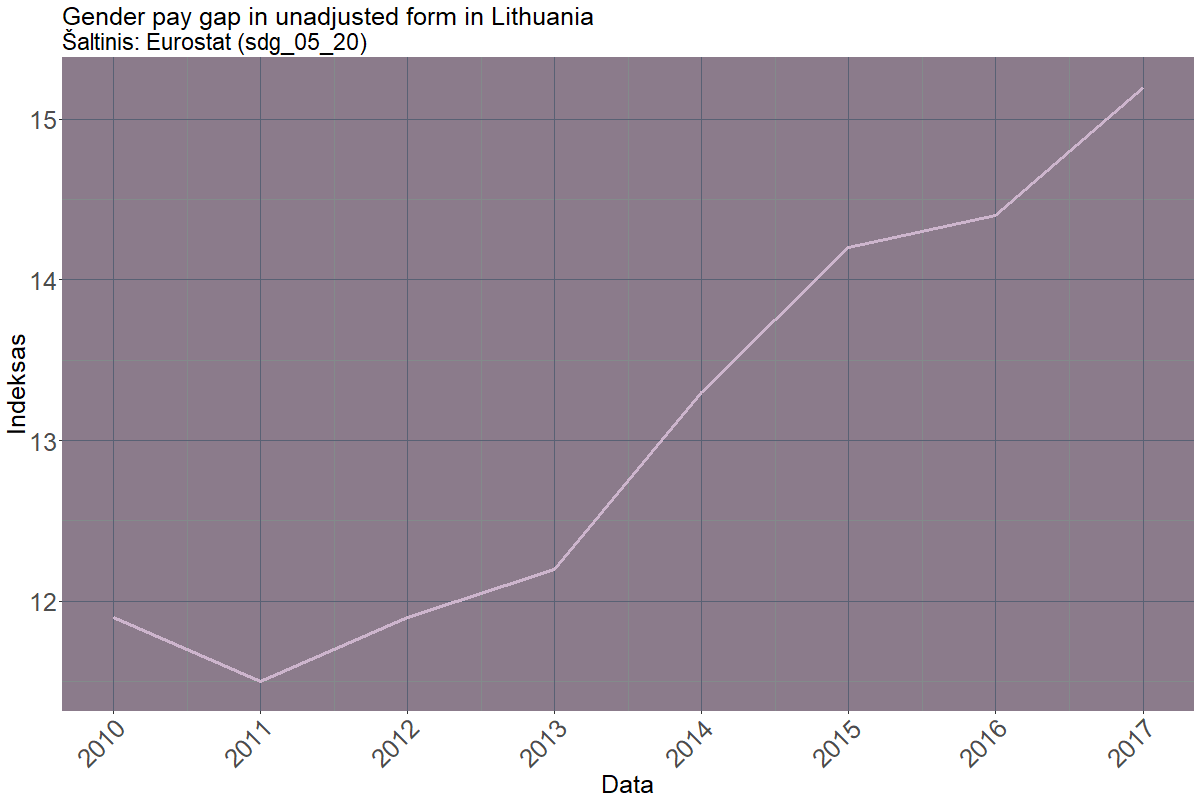
\includegraphics[scale=0.4]{paveiksliukas2.png}
\caption{Eurostat: „Gender pay gap in unadjusted form in Lithuania“}
\end{figure}

\item Lyčių diskriminacija šeimyninėje aplinkoje gali atsirasti ir dėl užimamų vyro ir moters pareigų darbe. Deja, „Pastebima, jog visame pasaulyje vyrai užima geresnes ir aukštesnes pozicijas“. Šis aspektas gali lemti pernelyg didelį vyrų pasitikėjimą savimi, dėl kurio yra nuvertinamos moterys. Vyrai, jausdamiesi valdingi savo karjeroje, to paties siekia ir kitose gyvenimo srityse, todėl, esant galimybei, linkę dominuoti. 

\item Būtina paminėti ir užimtumo lygio skirtumą tarp vyrų ir moterų. Remiantis EUROSTAT duomenimis, pastaruoju mietu Lietuvoje vyrų ir moterų užimtumo  lygio skirtumas mažėja – „užimtumo sritis, nors ir tendencingai, gerėja kiekybine prasme, vis dėl to išlieka dar pakankamai diskriminuojanti“. Lietuvos statistikos departamento duomenimis, moterų neužimtumas yra didesnis. Manoma, kad labiausias tai yra susiję su moterų išgyvenama dilema arba nelygybe, verčiančia rinktis tarp šeimos ir karjeros. Moterys bando ne tik pažinti save, atrasti patinkančią veiklos sritį, gerai apmokamą darbą, bet ir gimdo, prižiūri, augina vaikus, atsako už namų ruošą. Kadangi išvardyti dalykai yra laikomi vidinės sferos arba asmeninio gyvenimo dalimi, jie yra ne tiek reikšmingi visuomenei kaip, pavyzdžiui, besikeičiantys ekonomikos veiksniai. Tokiu būdu, skirtumas tarp moterų ir vyrų užimtumo lygiu nesparčiai juda pagerėjimo link.

\begin{figure}[H]
\captionsetup{justification=centering}
\center
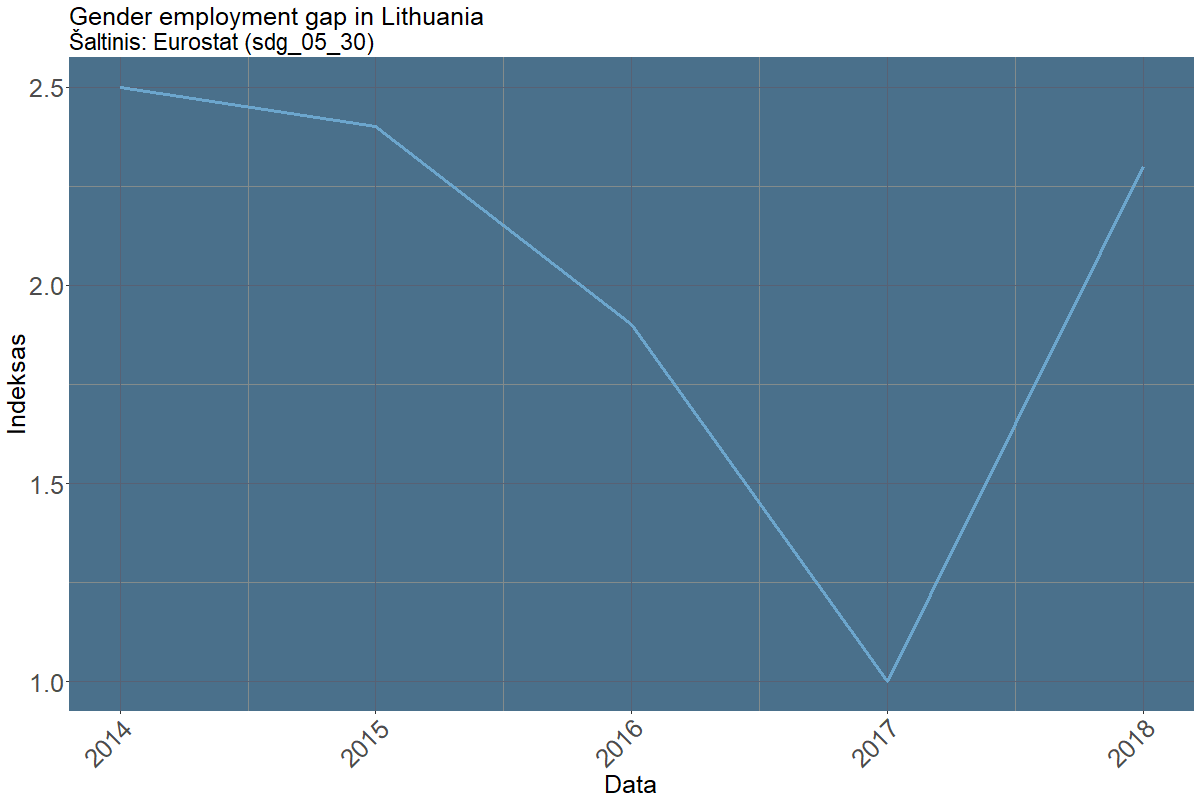
\includegraphics[scale=0.4]{paveiksliukas3.png}
\caption{Eurostat: Gender pay gap in Lithuania}
\end{figure}

\begin{figure}[H]
\captionsetup{justification=centering}
\center
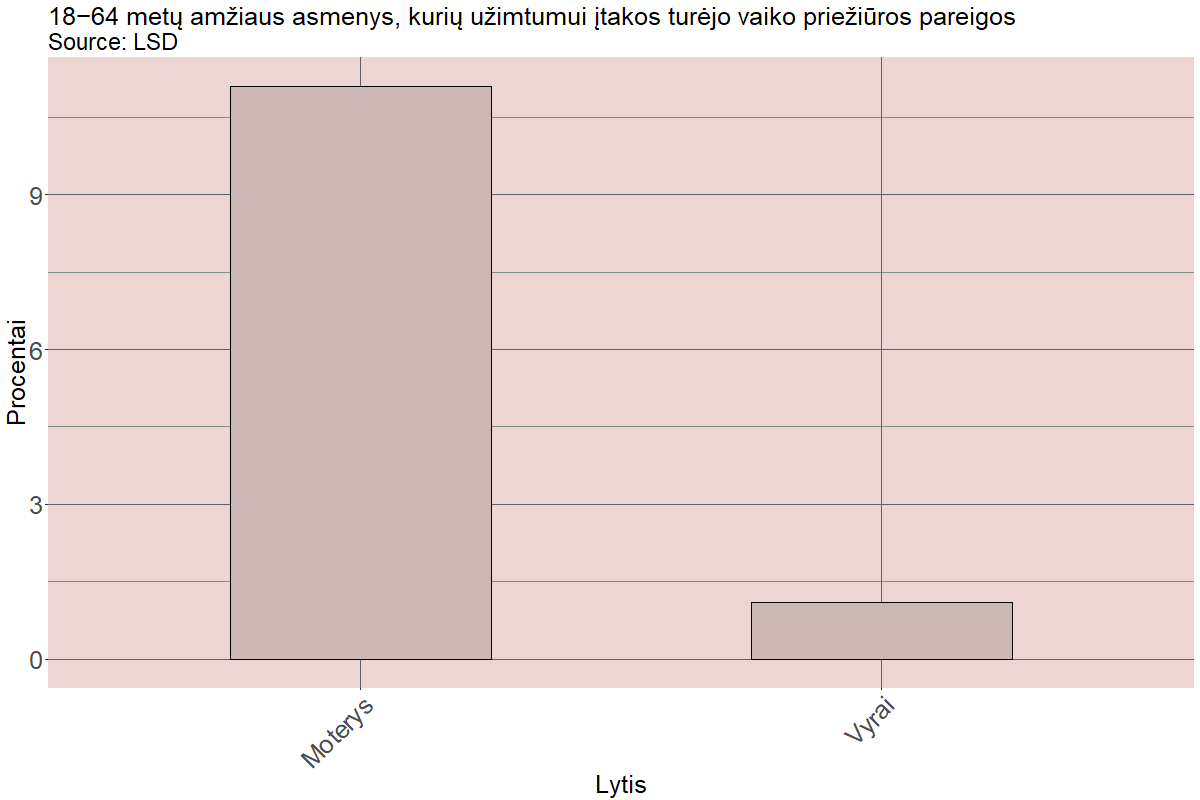
\includegraphics[scale=0.4]{paveiksliukas4.png}
\caption{Lietuvos statistikos departamentas: 18-64 metų amžiaus asmenys, kurių užimtumui įtakos turėjo vaiko priežiūros pareigos}
\end{figure}

\end{enumerate}

\section{Išvados}
Lyčių nelygybės problema turi būti nagrinėjama ir sprendžiama šiuolaikinėje visuomenėje. Lygybė yra vienas iš varomųjų variklių, palaikančių stabilumą skirtingose gyvenimo srityse: asmeniniame gyvenime, ekonomikoje, darbo rinkoje ir kt. Todėl yra būtina analizuoti kuo daugiau būdu, kurie galėtų padėti judėti link moterų ir vyrų lygybės. 
\begin{enumerate}
\item Vienas efektyviausių būdu mažinant lyčių nelygybės problemą yra visuomenės mentaliteto performavimas. Žmonės neturi būti ugdomi pagal moterims ir vyrams skirtus vaidmenis. Nuostatas, kad moterys yra priskiriamos vidinei sferai, o vyrai – išorinei, turi būti pakeistas. Visuomenei privalu įsisavinti faktą, kad jokia lytis neturi būti diskriminuojama – moterys ir vyrai yra lygūs visose gyvenimo srityse.
\item Darbo užmokesčio skirtumas turi būti mažinamas. Kiekvienas darbas gali būti kokybiškai atliktas kiekvienos lyties atstovo. Privalu atsižvelgti ne į samdomo žmogaus lytį, o į jo kompetentingumą, profesionalumą, gebėjimą kritiškai mąstyti. Darbo profesionalais gali būti tiek moterys, tiek vyrai.
\item Šeimoje dviejų lyčių atstovai jokiu būdu negali būti diskriminuojami. Abu, moteris ir vyras, kuria bendrą visuomenės dalį, ją puoselėja ir papildo vienas kitą. Tačiau dauguma žmonių nesuvokia „lyčių papildomumo“ sąvokos ir mano, kad tai yra tam tikras darbų ir kitų veiklų paskirstymas tarp moters ir vyro. Deja, tai dažniausiai nulemia lyčių nelygybę šeimyniniuose santykiuose. Tokiu būdu, visuomenė turi priimti ir įsisavinti kitokią „lyčių papildomumo“ reikšmę, grindžiamą moterų ir vyrų bendradarbiavimu ir lygybe visose veiklose – jie abu rūpinasi šeima.
\item Tam, kad lyčių nelygybė sumažėtų ir šeimose, privalu skatinti tėvus kuo dažniau  laiko skirti šeimos buičiai, pavyzdžiui, auginant vaikus. Kadangi „rūpinimasis buitimi vis dar laikomas neapmokamu darbu, todėl daugelis šalių pradėjo priiminėti įstatymus, stengdamosi motyvuoti tėvus labiau rūpintis šeima, kad moterys lengviau grįžtų į darbą“. Tokiu būdu, moterys galėtų greičiau atsikratyti karjeros spragų ir užimti panašaus lygio darbo pareigas kaip ir vyrai. Tai galėtų sumažinti lyčių nelygybė tiek darbo sferoje, tiek šeimos.
\end{enumerate}
Be abejo yra dar daugiau būdu, galinčių pamažu mažinti lyčių nelygybę. Tačiau visi jie turi būti skleidžiami ir puoselėjami, kadangi net ir „Kiekvienas vyras motinos įsčiose prasideda kaip mergaitė“ \cite{vanagaite2017jis} ). Todėl lyčių nelygybės visuomenėje egzistavimas yra tiesiog nepriimtinas.
\section{Literatūros sąrašas}
\nocite{*}
\printbibliography[title={Naudota literatūra}]

\end{document}